\documentclass[11pt,twoside,letterpaper]{book}
\usepackage{longtable}
\usepackage{multirow}
\usepackage{xltxtra}


\usepackage{pdflscape}
\usepackage{etoolbox}
\usepackage{tocloft}

\usepackage[bookmarksnumbered, bookmarksopen=true]{hyperref}
\hypersetup{colorlinks,
  linkcolor=blue,
  linktoc=page}

\usepackage{amsmath}
\usepackage{microtype}
%para codigo fuente
\usepackage{color}
\usepackage{xcolor}
\usepackage{listings}

\usepackage{bookmark}
\bookmarksetup{numbered}

\usepackage{titlesec} %reformatting the chapter headings
\titleformat{\chapter}[block]
{\normalfont\LARGE\bfseries\centering}
{CAPITULO \thechapter: }{0em}{}

\makeatletter
\bookmarksetup{%
  addtohook={%
    \ifnum\toclevel@chapter=\bookmarkget{level}\relax
    \renewcommand*{\numberline}[1]{Capítulo #1: }%
    \fi
  },
}
\makeatother

\renewcommand{\lstlistingname}{Listado}

\lstset{
  basicstyle=\footnotesize\ttfamily,
  language=C++
}

%margenes

%segun guia
\usepackage[top=2cm, bottom=2cm, inner=3cm, outer=2cm]{geometry}

%segun CD de carrera
%\usepackage[top=2.5cm, bottom=2.5cm, inner=3.5cm, outer=2.5cm]{geometry}

% quita la sangria a los parrafos (sin sangria se ve feo :-)
%\setlength{\parindent}{0cm}

% Para tener cabecera y pie de página con un estilo personalizado
\usepackage{fancyhdr}

% Espacio parrafos
\setlength{\parskip}{6pt}
\usepackage{adjustbox}

\usepackage{graphicx}
\usepackage{pstricks}
% Todas las imágenes están en el directorio tp-img:
\newcommand{\imgdir}{img}
\graphicspath{{\imgdir/}}

\usepackage{fontspec}
\usepackage{polyglossia}
\setmainlanguage{spanish}

\setromanfont[Mapping=tex-text]{Linux Libertine O}
\setsansfont[Mapping=tex-text]{DejaVu Sans}
\setmonofont[Mapping=tex-text]{DejaVu Sans Mono}

\title{Mejoramiento del Proceso de deshidratación mediante la construcción de un
  sistema de control automático}
\author{Daniel Rodrigo Saguez Tezanos Pinto}
\date{Diciembre, 2015}

\begin{document}
  %
  % caratula
  %
  %para poner bookmark del CD de requisitos
  \bookmark[page=1,level=-2]{INICIO}

  \pagenumbering{Roman} % para comenzar la numeracion de paginas en numeros romanos

  % caratula --------------------------------------------------------------
  \newcommand{\umsslogo}{%
    \adjustbox{valign=t}{
\includegraphics[scale=0.04]{umss}}%
  }
  \newcommand{\fcytlogo}{%
    \adjustbox{valign=t}{
\includegraphics[scale=0.1]{fcyt}}%
  }

  % Carátula:
  \makeatletter
  \begin{titlepage}
    \thispagestyle{empty}

    \begin{tabular}[t]{c p{10cm} c}
      \umsslogo &
      \begin{center}
        \large{\textsc{Universidad Mayor de San Simón }} \\
        \large{\textsc{Facultad de Ciencias y Tecnología }} \\
        \large{\textsc{Carrera de Ingeniería en Informática}}
      \end{center}
      &
      \fcytlogo \\
    \end{tabular}
    \vfill

    \begin{center}
      \huge{\textsc{\@title}}
    \end{center}
    \vspace{0.5cm}

    %\begin{flushright}
    \begin{center}
      \textsc{
        Proyecto de grado, presentado para optar\\
        al Diploma Académico de Licenciatura \\
        en Ingeniería en Informática.
      }
      %\end{flushright}
    \end{center}

    \vfill
    \begin{tabbing}
      \hspace{2cm}\=\+
      \textsc{Presentado por:} \@author    \\
      \\
      \textsc{Tutor:} MA Leticia Blanco Coca    \\
      \\
      %\textsc{Cochabamba - Bolivia}\\
      \\
    \end{tabbing}

    \begin{center}
      \textsc{Cochabamba - Bolivia}\\
      \textsc{\@date}
    \end{center}

    \vfill

    %\hrule
    %\vspace{0.2cm}
    %\noindent\small{Trabajo de Grado \hfill}

  \end{titlepage}

  % caratula --------------------------------------------------------------

  %Dedicatoria y agradecimientos
\addcontentsline{toc}{chapter}{Dedicatoria}
\chapter*{}
\begin{flushright}
\textit{Dedicado a \\
    Valery Tamara Saguez Lamas \\
    Cristal Amalia Tezanos Pinto Solares}
    \end{flushright}
\newpage


  \addcontentsline{toc}{chapter}{Agradecimientos}
\chapter*{}
\begin{flushright}
\textit{La realizaci�n de este proyecto de grado \\
        blah blah blah blah blah blah blah blah \\
        blah blah blah blah blah blah blah blah \\
        blah blah blah blah blah blah blah blah \\ 
        blah blah blah blah blah blah blah blah \\
        }
    \end{flushright}
\newpage


  % Las páginas empiezan a contar desde aqui
  \setcounter{page}{1}
  \addcontentsline{toc}{chapter}{Ficha resumen}
\chapter*{Ficha resumen}
Se busca mejorar el proceso de deshidratación de alimentos, mediante la
conjunción de un sistema eléctrico/electrónico, sensores, controladores y
microcontroladores; que permitan tener un seguimiento automático del proceso de
deshidratado, con el fin de monitorear las variables referentes al secado de
diferentes tipos de alimentos; variables como temperatura, velocidad de flujo de
aire, peso, humedad del aire, humedad del producto.
\cleardoublepage

  \bookmark[page=9,level=-1]{�ndice general}
% Pongo el �ndice en una p�gina aparte:
\tableofcontents
\cleardoublepage

  \listoffigures % indice de figuras
\cleardoublepage

  \listoftables % indice de tablas

  \chapter{Introducción}\label{cap:intro}
\pagenumbering{arabic}
\section{Antecedentes}
El  Programa de Alimentos y Productos Naturales (PAPN) fue creado el 13 de
febrero de 1987 como un programa, pero rápidamente se convirtió, por iniciativa
y esfuerzo de su dirección y sus miembros, en un centro superior de
investigación. Este centro depende de la Facultad de Ciencias y Tecnología de la
Universidad Mayor de San Simón (UMSS) y esta situado en el campus principal.
Dentro de sus actividades de ciencia y tecnología en el campo agroalimentario y
de productos naturales, la UMSS ejecuta la investigación a través de convenios y
proyectos en diferentes ámbitos del desarrollo regional y nacional, a través del
centro superior PAPN.

De acuerdo a posibilidades y disponibilidades, se han incorporado al PAPN
practicas sobre secado y análisis sensorial para los estudiantes de ingeniería
industrial y alimentos, así como se han realizado diversos estudios en el secado
de alimentos andinos y el diseño de secadores solares, convencional, deseando
implementar 2 nuevos tipos de deshidratadores: cama fluidizada. y spray.

En este sentido, para mejorar el estudio y la investigación del secado de
alimentos es que este centro precisa la construcción de tres secadores
experimentales automatizados que permitan obtener datos de las variables de
secado de diferentes tipos de alimentos de la forma más rápida y precisa.

El propósito de un control automático en un sistema es producir una salida
deseada cuando las entradas del sistema son modificadas. Estas entradas se
modifican por señales de mando, y también por perturbaciones, que se espera que
el control automático minimice.

%\pagebreak % poner esto al final de cada seccion
\section{Identificación del problema}

Es complicado analizar todas las variables que intervienen en el proceso de
deshidratado, para que, dado un producto que se desea secar; se pueda escoger el
mejor proceso para este producto.

\subsection{Definición del problema}

¿Como mejorar la obtención y análisis de las variables de secado, de distintos
tipos de alimentos, por medio del control de las variables de entrada?

\section{Objetivos}

\subsection{Objetivos General}
\begin{itemize}
  \item Construir un sistema de control automático para el proceso de
        deshidratación experimental de alimentos.
  %\item blah blah blah blah.

\end{itemize}

\subsection{Objetivos Específicos}
Los objetivos a cumplir durante el desarrollo del proyecto son:
\begin{itemize}
  \item Determinar el modelo del sistema y de control.
  \item Seleccionar sensores, controladores y actuadores a utilizar.
  \item Desarrollar el modulo para funcionamiento básico del microcontrolador.
  \item Diseñar el modelo unificado el sistema electrónico y el sistema de
        información.
  \item Desarrollar el modulo de control supervisado.
  \item Desarrollar el modulo de cambio de parámetros de control.
  \item Implementar el control automático.
\end{itemize}

\section{Alcance}
El proyecto tendrá el siguiente alcance:
\begin{itemize}
  \item Sistema electrónico de control.
  \item Sistema informático de análisis y seguimiento del proceso de secado.
\end{itemize}

%\pagebreak % poner esto al final de cada seccion
\section{Justificación}
La desecación de vegetales por paso de aire caliente sobre superficie húmeda,
representa la forma mas común de secado de vegetales destinados a la
alimentación, siendo uno de los procesos mas antiguos de conservación que se
conocen.

Mediante este método es posible preservar el color, los principios activos otras
características de calidad que se pierden por acción de las encimas después de
la cosecha, permitiendo de esta manera, una mejor conservación por tiempos
relativamente largos sin perdidas de estas características.

Ante la necesidad de conocer las distintas cualidades y capacidades de los
distintos tipos de deshidratadores, y de obtener los cambios de sus variables
durante el proceso de deshidratación de manera rápida y casi desatendida por una
persona se ve que es conveniente la construcción de un sistema de control
automático para cada tipo de deshidratador que se cuenta en la planta piloto.



  \include{009-Deshidratación}
  \include{010-ControlAutomático}
  \chapter{Herramientas}
\section{Arduino}

Es una plataforma de hardware libre, basada en una placa con un microcontrolador
y un entorno de desarrollo, diseñada para facilitar el uso de la electrónica en
proyectos multidisciplinares.

El hardware consiste en una placa con un microcontrolador Atmel AVR y puertos de
entrada/salida. Los microcontroladores más usados son los Atmega168, Atmega328,
Atmega1280, y Atmega8 por su sencillez y bajo coste, que permiten el desarrollo
de múltiples diseños. Por otro lado el software consiste en un entorno de
desarrollo que implementa el lenguaje de programación «Processing/Wiring» y el
cargador de arranque(bootloader) que es ejecutado en la placa. Se programa en el
ordenador para que la placa controle los componentes electrónicos.

Desde octubre de 2012, Arduino utiliza los microcontroladoras CortexM3 de ARM de
32 bits, que coexistirán con las más limitadas, pero también económicas AVR de 8
bits. ARM y AVR no son plataformas compatibles a nivel binario, pero se pueden
programar con el mismo IDE de Arduino y hacerse programas que compilen sin
cambios en las dos plataformas. Eso sí, los microcontroladores CortexM3 usan
3,3V, a diferencia de la mayoría de las placas con AVR, que generalmente usan
5V. Sin embargo, ya anteriormente se lanzaron placas Arduino con Atmel AVR a
3,3V como la Arduino Fio y existen compatibles de Arduino Nano y Pro como
Meduino en que se puede conmutar el voltaje.

De la placa Arduino, puede tomar información del entorno a través de sus
entradas analógicas y digitales, puede controlar luces, motores y otros
actuadores. El microcontrolador en la placa Arduino se programa mediante el
lenguaje de programación Arduino (basado en Wiring) y el entorno de desarrollo
Arduino (basado en Processing). Los proyectos hechos con Arduino pueden
ejecutarse sin necesidad de conectar a un ordenador.

También cuenta con su propio software que se puede descargar de su página
oficial que ya incluye los drivers de todas las tarjetas disponibles lo que hace
más fácil la carga de códigos desde el computador.

También se puede utilizar para desarrollar objetos interactivos autónomos o
puede ser conectado a software tal como Adobe Flash, Processing, Max/MSP, Pure
Data. Una tendencia tecnológica es utilizar Arduino como tarjeta de adquisición
de datos desarrollando interfaces en software como JAVA, Visual Basic y LabVIEW
6 . Las placas se pueden montar a mano o adquirirse. El entorno de desarrollo
integrado libre se puede descargar gratuitamente.

\subsection{Arduino Mega 2560}
El Arduino Mega 2560 esta basado en el Atmega2560. Cuenta con 54 pines digitales
de entrada / salida (de los cuales 15 se pueden utilizar como salidas PWM), 16
entradas analógicas, 4 UARTs (hardware puertos serie), un oscilador de 16 MHz,
una conexión USB, un conector de alimentación, un conector ICSP(In Cirtuit
Serial Programmer), y un botón de reinicio. Contiene todo lo necesario para
apoyar el microcontrolador; simplemente conectarlo a un ordenador con un cable
USB o el poder con un adaptador de CA o la batería a CC para empezar. El
conector Mega 2560 es compatible con la mayoría de los escudos diseñados para el
Arduino Uno y los antiguos tableros Duemilanove o Diecimila.

El Mega 2560 es una actualización de la Arduino Mega, que sustituye.

\subsubsection{Caracteristicas}
\begin{description} \itemsep0pt \parskip0pt \parsep0pt
  \item[Microcontrolador] Atmega2560
  \item[Voltaje de funcionamiento] 5V
  \item[Voltaje de entrada (recomendado)] 7-12V
  \item[Voltaje de entrada (límite)] 6-20V
  \item[Pines Digitales E/S] 54 (de los cuales 15 proporcionan salida PWM)
  \item[Entradas analógicas] 16
  \item[Corriente DC por cada pin E/S] 20 mA
  \item[Corriente DC de el pin 3.3V] 50 mA
  \item[Memoria Flash] 256 KB de los cuales 8 KB utilizado por el gestor de arranque
  \item[SRAM] 8 KB
  \item[EEPROM] 4 KB
  \item[Frecuencia] 16 MHz
  \item[Longitud] 101,52 mm
  \item[Ancho] 53.3 mm
  \item[Peso] 37g
\end{description}

\subsection{Processing} Es un lenguaje de programación y entorno de desarrollo
integrado de código abierto basado en Java, de fácil utilización, y que sirve
como medio para la enseñanza y producción de proyectos multimedia e interactivos
de diseño digital. Fue iniciado por Ben Fry y Casey Reas a partir de reflexiones
en el Aesthetics and Computation Group del MIT Media Lab dirigido por John
Maeda.

Se distribuye bajo la licencia GNU GPL.

\subsubsection{Alcance}

Al estar basado en Java, puede heredar todas sus funcionalidades, convirtiéndose
en una herramienta poderosa a la hora de encarar proyectos complejos.

%\begin{table}
%\centering
%  \begin{tabular}{r r r r}
%\textbf{Pin} & \textbf{Descripción} & \textbf{Pin} & \textbf{Descripción} \\
%\hline
%1 & \texttt{3.3v} & 2 & \texttt{5v} \\
%3 & \texttt{SDA0*} & 4 & \texttt{5v} \\
%5 & \texttt{SCL0*} & 6 & \texttt{GND} \\
%7 &  \texttt{GPIO\_GCLK} & 8 & \texttt{TXD0*} \\
%9 &  \texttt{GND} & 10 & \texttt{RXD0*} \\
%11 &  \texttt{GPIO\_GEN0} & 12 & \texttt{GPIO\_GEN1} \\
%13 &  \texttt{GPIO\_GEN2} & 14 & \texttt{GND} \\
%15 &  \texttt{GPIO\_GEN3} & 16 & \texttt{GPIO\_GEN4} \\
%17 &  \texttt{3.3v} & 18 & \texttt{GPIO\_GEN5} \\
%19 &  \texttt{SPI\_MOSI*} & 20 & \texttt{GND} \\
%21 &  \texttt{SPI\_MISO*} & 22 & \texttt{GPIO\_GEN6} \\
%23 &  \texttt{SPI\_SCLK*} & 24 & \texttt{SPI\_CEO\_N*} \\
%25 &  \texttt{GND} & 26 & \texttt{SPI\_CE1\_N*} \\
%  \end{tabular}
%  \caption{Descripción de los pines de GPIO}
%  \label{table:gpio_descr}
%\end{table}

\section{Conclusiones}

Se opto por la tecnología de Arduino por la simplicidad de desarrollo y las
capacidades que exceden a los requerimientos actuales. Se escogió el Arduino
Mega 2560, por su bajo coste y la cantidad extendida de pines, tanto analógicos
como digitales

  \chapter{Metodología}

\section{Pila de productos (product backlog)}
%\section{Pila del producto}
En el presente proyecto se utilizará la metodología de desarrollo de software
SCRUM \cite{scrum_book}.

La siguiente tabla es una lista priorizada de requisitos (características) para
ser implementadas en el proyecto. Cada una de estas características se
escribieron de acuerdo a los objetivos específicos, que fueron definidos en el
Capitulo \ref{cap:intro}.

\def\arraystretch{2}
\newcommand{\pbtemp}{Como investigador deseo conocer la temperatura más adecuada para realizar el deshidratado. }


\begin{longtable}{|c|p{12.5cm}|c|} %p{1.8cm}|p{1.9cm}
\hline
\textbf{N°} & \textbf{Características } & \textbf{Prioridad} \\ \hline
\hline

1 & \pbtemp & Alta  \\ \hline
\end{longtable}

\section{Estimación de historias de usuario}
La estimación de esfuerzo de las historias de usuario se realizaran utilizando
la técnica de Planning Poker. Se utilizara el rango de 1, 2, 3, 5, 8, 13, 21, 34.

\section{Ciclo Inicial(Sprint A) }
El ciclo inicial empiezo el día Viernes 26 de Septiembre del 2014. Este ciclo
consta de 2 semanas para completar las historias que serán definidas en la
planificación del sprint. El ciclo concluirá el Jueves 9 de Octubre del 2014.

%\begin{landscape}
\subsection{Pila del Ciclo (Sprint backlog)}
En este ciclo se eligió trabajar en las características 1 y 2 de la pila de
productos, por el hecho de tener alta prioridad. Cada característica se divide
en historias de usuario, y estas son estimadas con puntos de historia. En los
Cuadros \ref{table:eus1} y \ref{table:eus2} se definen las estimaciones. Para
cada historia de usuario se definen criterios de aceptación, como se muestra en
el Cuadro~\ref{table:criteriosSA}.

Cada historia de usuario se divide en tareas, y se definen en los Cuadros
\ref{table:tareasUS1}, \ref{table:tareasUS2} y \ref{table:tareasUS3_1}.

%--------------------------------------------------------------------
\begin{table}[ht]
\centering
\begin{tabular}{|l|p{6cm}|c|p{5cm}|r|}
\hline
\textbf{No.} & \textbf{Feature} & \textbf{Id.} & \textbf{Historia de usuario} & \textbf{Estimación} \\
\hline
1 & \pbtemp & US1 & Controlar Temperatura. & 3 \\
\hline
\end{tabular}
\caption{Estimación de US1}
\label{table:eus1}
\end{table}

%--------------------------------------------------------------------

\subsection{Demostración de fin de sprint}


\subsection{Gráfico burn down del sprint}
La Figura~\ref{fig:sprintA} muestra el gráfico \emph{burn down} del presente
sprint.

\subsection{Retrospectiva del sprint}
\begin{itemize}
  \item ¿Qué salió bien?
    \begin{itemize}
        \item Se completaron la mayoria de las tareas de la iteración.
        \item Se escribieron pruebas de unidad para el código desarrollado.
    \end{itemize}

  \item ¿Qué podría haber sido mejor?
    \begin{itemize}
        \item La estimación de la historia US3 no fue buena.
    \end{itemize}

  \item ¿Qué  se puede mejorar en el futuro?
    \begin{itemize}
        \item Mejorar las estimaciones de las historias, si la historia es muy larga es mejor dividirla.
    \end{itemize}
\end{itemize}





  %\chapter{Conclusiones y Recomendaciones}
\section{Conclusiones}

blah blah blah blah blah blah blah blah blah blah blah blah blah blah blah blah blah blah blah blah  blah blah blah blah blah blah blah blah blah blah blah blah blah blah blah blah blah blah blah blah blah blah blah blah blah blah blah blah blah blah blah blah blah blah blah blah blah blah blah blah blah blah blah blah blah blah blah blah blah blah blah blah blah blah blah blah blah blah blah blah blah blah blah blah blah blah blah blah blah blah blah blah blah blah blah blah blah blah blah blah blah blah blah blah blah blah blah blah blah blah blah blah blah blah blah blah blah blah blah blah blah blah blah blah blah blah blah blah blah blah blah blah blah blah blah blah blah blah blah blah blah blah blah blah blah blah blah blah blah blah blah blah blah blah blah blah blah blah blah blah blah blah blah blah blah blah blah blah blah blah blah blah blah blah blah blah blah blah blah blah blah blah blah blah blah blah blah blah blah blah blah blah blah blah blah blah blah blah blah blah 

\section{Recomendaciones}


blah blah blah blah blah blah blah blah blah blah blah blah blah blah blah blah blah blah blah blah  blah blah blah blah blah blah blah blah blah blah blah blah blah blah blah blah blah blah blah blah blah blah blah blah blah blah blah blah blah blah blah blah blah blah blah blah blah blah blah blah blah blah blah blah blah blah blah blah blah blah blah blah blah blah blah blah blah blah blah blah blah blah blah blah blah blah blah blah blah blah blah blah blah blah blah blah blah blah blah blah blah blah blah blah blah blah blah blah blah blah blah blah blah blah blah blah blah blah blah blah blah blah blah blah blah blah blah blah blah blah blah blah blah blah blah blah blah blah blah blah blah blah blah blah blah blah blah blah blah blah blah blah blah blah blah blah blah blah blah blah blah blah blah blah blah blah blah blah blah blah blah blah blah blah blah blah blah blah blah blah blah blah blah blah blah blah blah blah blah blah blah blah blah blah blah blah blah blah blah blah 


\section{Posibles extensiones}


blah blah blah blah blah blah blah blah blah blah blah blah blah blah blah blah blah blah blah blah  blah blah blah blah blah blah blah blah blah blah blah blah blah blah blah blah blah blah blah blah blah blah blah blah blah blah blah blah blah blah blah blah blah blah blah blah blah blah blah blah blah blah blah blah blah blah blah blah blah blah blah blah blah blah blah blah blah blah blah blah blah blah blah blah blah blah blah blah blah blah blah blah blah blah blah blah blah blah blah blah blah blah blah blah blah blah blah blah blah blah blah blah blah blah blah blah blah blah blah blah blah blah blah blah blah blah blah blah blah blah blah blah blah blah blah blah blah blah blah blah blah blah blah blah blah blah blah blah blah blah blah blah blah blah blah blah blah blah blah blah blah blah blah blah blah blah blah blah blah blah blah blah blah blah blah blah blah blah blah blah blah blah blah blah blah blah blah blah blah blah blah blah blah blah blah blah blah blah blah blah 



  \begin{thebibliography}{99}
%\bibitem{Libro_ejemplo} Apellido, Nombre.Nombre texto.Editorial.A�o.# de pag
\bibitem{opencv_cookbook} Lagani�re, Robert.OpenCV 2 Computer Vision Application Programming Cookbook.Packt Publishing.2011.P\'agina 1
\bibitem{raspi_evilg} Norris, Donald.Raspberry Pi Projects for the Evil Genius.Mc Graw Hill.2014 . P�gina 22
\bibitem{prac_rob} Sahin, Ferat; Kachroo, Pushkin . Practical and Experimental Robotics . CRC Press . 2008 . P�gina 43
\bibitem{l298_data} STMicroelectronics . L298 DUAL FULL-BRIDGE DRIVER Datasheet. STMicroelectronics . 2000 . P�gina 2
\bibitem{comp_cv} J�hne, Bernd; Hau�ecker, Horst .  Computer Vision and Applications . Academic Press . 2000 . P�gina 1
\bibitem{appl_cmv} E. R. Davies . Computer and Machine Vision: Theory, Algorithms, Practicalities . Academic Press . 2012 . P�gina 10
\bibitem{modulosocv} Brahmbhatt, Samarth . Practical OpenCV . APress . 2013 . P�gina 22
\bibitem{tomografia} Nixon, Mark; Aguado, Alberto . Feature Extraction and Image Processing . Newnes . 2002 . P�gina 2
\bibitem{resonancia} Davies, E. Roy . Machine Vision: Theory, Algorithms, Practicalities . Morgan Kaufmann . 2005 . P�gina 53
\bibitem{interpolacion} Cyganek, Boguslaw; Siebert, J. Paul; An introduction to 3D computer vision techniques and algorithms . Wiley . 2009 . P�gina 412
\bibitem{noisereduc} E. R. Davies . Computer and Machine Vision: Theory, Algorithms, Practicalities . Academic Press . 2012 . P�gina 40
\bibitem{features} Nixon, Mark; Aguado, Alberto . Feature Extraction and Image Processing . Newnes . 2002 . P�gina 99
\bibitem{egomotion} Burger, Wilhelm; Bhanu, Bir . Estimating 3-D Egomotion from Perspective Image Sequences . IEEE . 2002 . P�gina 1
\bibitem{tracking} Lyudmila MIHAYLOVA; Paul BRASNETT; Nishan CANAGARAJAH; David BULL . Object Tracking by Particle Filtering Techniques in Video Sequences . Department of Electrical and Electronic Engineering, University of Bristol, UK . . P�gina 1
\bibitem{edgedetection} E. R. Davies . Computer and Machine Vision: Theory, Algorithms, Practicalities . Academic Press . 2012 . P�gina 112
\bibitem{cidetection} E. R. Davies . Computer and Machine Vision: Theory, Algorithms, Practicalities . Academic Press . 2012 . P�gina 149
\bibitem{camara} Wenczel, Norma .  Inside the Camera Obscura � Optics and Art under the Spell of the Projected Image . Max Planck Institute for the History of Science . 2007 . P�gina 13-30
\bibitem{luz_visible} Starr, Cecie . Biology: Concepts and Applications . Thomson Brooks/Cole . 2005 . P�gina 94
\bibitem{appl_cv} J�hne, Bernd y Hau�ecker, Horst . Computer Vision and Applications, A Guide for Students and Practitioners . Academic Press . 2000 . P�gina 564
\bibitem{cv_tasks} J�hne, Bernd y Hau�ecker, Horst . Computer Vision and Applications, A Guide for Students and Practitioners . Academic Press . 2000 . P�gina 7
\bibitem{filtros} Bhat, Pravin . Gradientshop: A gradient-domain optimization framework for image and video filtering . ACM Transactions on Graphics . 2010 . P�gina 10  
\bibitem{restauracion} M. Bertalm�o, G. Sapiro, V. Caselles and C. Ballester. Image Inpainting . Proceedings of SIGGRAPH 2000 . 2000 . P�gina 1 
\bibitem{ipolinomica}  Agarwal, R.P.; Wong, J.Y. Patricia . Error Inequalities in Polynomial Interpolation and Their Applications . Springer Science+Bussiness Media, B.V. 1993 . P�gina 217
\bibitem{burndown} Cohn, Mike . User Stories Applied, for Agile Software Development . Addison-Wesley . 2004 . P�gina 121

%\bibitem{} . . . . P�gina 

%\bibitem{PHP} PHP Web-Seite: \url{http://www.php.net}

%\bibitem{robotica_wiki} Rob�tica - Wikipedia: \url{http://es.wikipedia.org/wiki/Rob�tica}. 25 de Marzo de 2014
\bibitem{robotica_wiki} Bermejo, Sergi . Desarrollo de robots basados en el comportamiento . Ediciones UPC . 2003 . P�ginas 26, 27
%\bibitem{opencv_wiki} OpenCV - Wikipedia: \url{http://en.wikipedia.org/wiki/OpenCV}. 25 de Marzo de 2014
\bibitem{scrum_book} Sutherland, Jeff . The Scrum Handbook . Scrum, Inc . 2001 . P�gina 6
\bibitem{opencv_oficial} P�gina oficial de OpenCV: \url{http://opencv.org/}. 27 de Marzo de 2014
\bibitem{raspberry_pi} P�gina oficial de Raspberry Pi: \url{http://www.raspberrypi.org/}. 27 de Marzo de 2014
\bibitem{raspberry_pi_wiki} Componentes de Raspberry Pi: \url{https://www.raspberrypi.org/blog/new-graphic/}. 8 de Septiembre de 2015
%\bibitem{single_board_pc} Single board computer - Wikipedia: \url{https://en.wikipedia.org/wiki/Single-board_computer}. 27 de Marzo de 2014
%\bibitem{reg_voltaje} Regulador de tensi�n: \url{https://es.wikipedia.org/wiki/Regulador_de_tensi\%C3\%B3n}. 11 de Septiembre de 2014
%\bibitem{bateria} Bater�a de ion de litio \url{https://es.wikipedia.org/wiki/Bater\%C3\%ADa_de_ion_de_litio}. 11 de Septiembre de 2014 
\bibitem{camera_mod} Raspberry Pi camera module: \url{http://www.raspberrypi.org/products/camera-module/}. 11 de Septiembre de 2014
\bibitem{cam_espec} Raspberry Pi camera module stock lens characteristics \url{http://www.truetex.com/raspberrypi} . 9 de Octubre de 2014
%\bibitem{camara} C�mara oscura \url{http://es.wikipedia.org/wiki/C\%C3\%A1mara_oscura} . 19 de octubre de 2014
%\bibitem{luz_visible} Radiaci�n electromagn�tica - Wikipedia\url{http://es.wikipedia.org/wiki/Radiaci\%C3\%B3n\_electromagn\%C3\%A9tica#Luz_visible} . 19 de octubre de 2014
%\bibitem{appl_cv} Applications for computer vision - Wikipedia \url{http://en.wikipedia.org/wiki/Computer_vision#Applications_for_computer_vision} . 20 de octubre de 2014
%\bibitem{cv_tasks} Typical tasks of computer vision - Wikipedia \url{http://en.wikipedia.org/wiki/Computer_vision#Typical_tasks_of_computer_vision} . 21 de octubre de 2014
%\bibitem{filtros} Procesamiento digital de im�genes - Wikipedia \url{http://es.wikipedia.org/wiki/Procesamiento_digital_de_im\%C3\%A1genes#Tipos} . 23 de octubre de 2014
%\bibitem{restauracion} Restauraci�n de imagen - Wikipedia \url{http://es.wikipedia.org/wiki/Restauraci\%C3\%B3n_de_imagen#Algoritmo} . 23 de octubre de 2014
%\bibitem{lrangefinder} Laser rangefinder - Wikipedia \url{http://en.wikipedia.org/wiki/Laser_rangefinder} . 23 de octubre de 2014
\bibitem{overclock} Introducing turbo mode: up to 50\% more performance for free \url{http://www.raspberrypi.org/introducing-turbo-mode-up-to-50-more-performance-for-free/} . 30 de octubre de 2014
\bibitem{raspicamimg} The Official Raspberry Pi Camera Module \url{http://www.raspberrypi-spy.co.uk/2013/05/the-official-raspberry-pi-camera-module/} . 5 de noviembre de 2014
\bibitem{tamiyawt} Tamiya Track and Wheel Set \url{http://www.superdroidrobots.com/shop/item.aspx/tamiya-track-and-wheel-set/409/} . 5 de noviembre de 2014
%\bibitem{ipolinomica} Polynomial interpolation \url{http://en.wikipedia.org/wiki/Polynomial_interpolation} . 4 de Enero del 2015
\bibitem{sensorccd} CCD and CMOS sensors \url{http://www.issibern.ch/forads/sr-009-23.pdf} . 09 de Septiembre del 2015
\end{thebibliography}

  %%\begin{titlepage}
\chapter*{}
\pagestyle{plain}

\begin{center}
\Huge{\textsc{Anexos}}
\end{center}

\addcontentsline{toc}{chapter}{Anexos}
%\end{titlepage}

\chapter*{}

\pagestyle{myheadings}
\markboth{ANEXOS}{ANEXO A}

\addcontentsline{toc}{section}{Anexo A: C�digo fuente}
\section*{Anexo A: C�digo fuente}
\subsection*{Clase para permitir movimiento aut�nomo al robot}
\lstinputlisting[language=c++, title={BaseCon.cpp}]{021-Anexo02-BaseCon.cpp}

\subsection*{Clase con la funci�n de reconocer obst�culos en el plano}
\lstinputlisting[language=c++, title={Blobs.cpp}]{022-Anexo03-Blobs.cpp}
\lstinputlisting[language=c++, title={Blobs.hpp}]{023-Anexo04-Blobs.hpp}

\subsection*{Clase que representa al sensor MPU6050}
Esta clase se ocupa de inicializar al sensor y obtener los �ngulos de inclinaci�n del Robot.
\lstinputlisting[language=c++, title={Giro.cpp}]{024-Anexo05-Giro.cpp}

\subsection*{Utilitarios}
En este archivo se encuentran las funciones \texttt{calcular\_distancia()} y \texttt{calcular\_distancia\_horizontal()}, que calculan la distancia vertical y horizontal de un objeto detectado en el plano. Tambi�n se encuentra la funci�n \texttt{leerConfigFile()}, que sirve para leer archivos de configuraci�n.

\lstinputlisting[language=c++, title={Utils.cpp}]{025-Anexo06-Utils.cpp}

\markboth{ANEXOS}{ANEXO B}
\addcontentsline{toc}{section}{Anexo B: Fotos del Robot}
\section*{Anexo B: Fotos del Robot}
%Robot con todos sus componentes instalados.

\begin{figure}
    \centering
    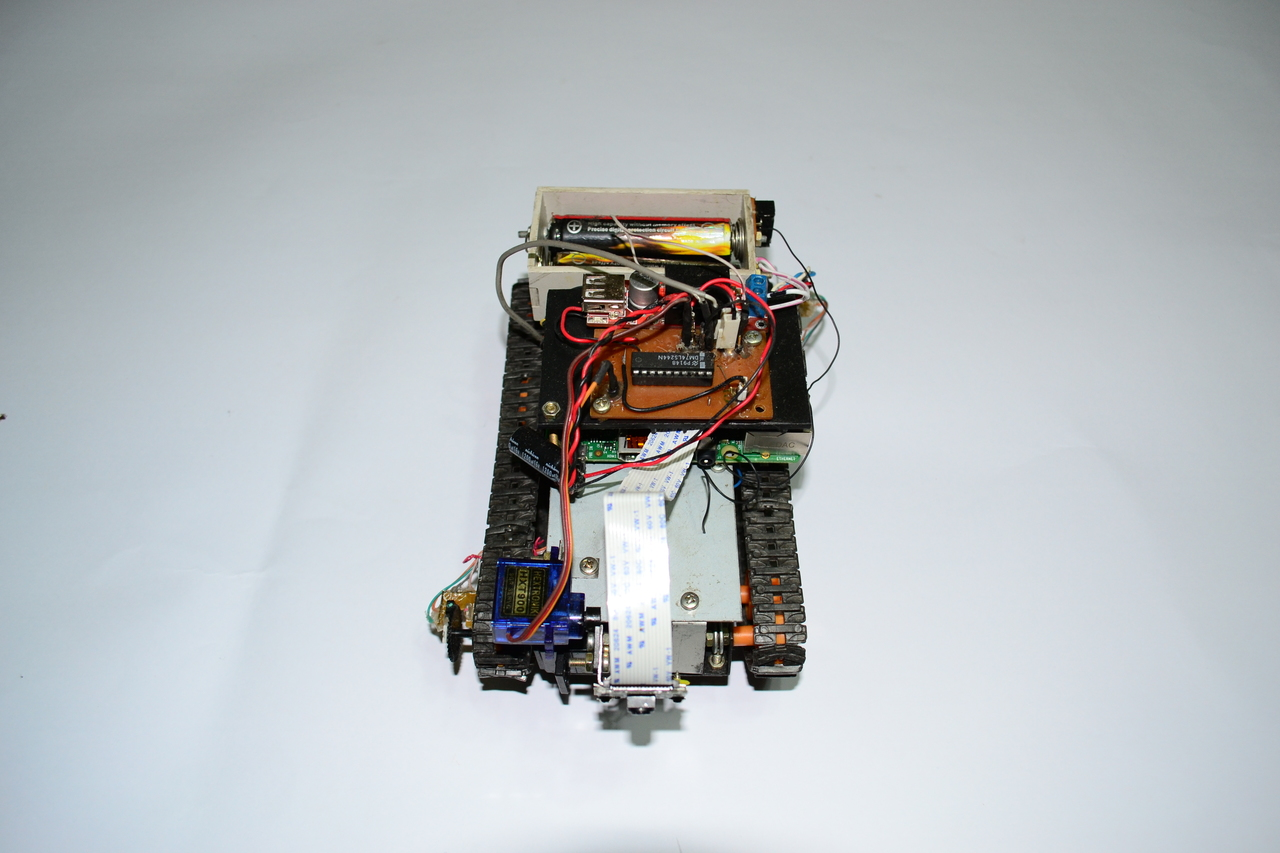
\includegraphics[width=0.8\textwidth]{r-DSC_0009.JPG}
    \caption{Vista frontal del robot. Se observa: el distribuidor de energ�a y regulador de voltaje al centro.}
\end{figure}

\newpage
\markboth{ANEXOS}{ANEXO C}
\addcontentsline{toc}{section}{Anexo C: Planilllas de seguimiento de sprint}
\section*{Anexo C: Planilllas de seguimiento de sprint}

\begin{table}
\centering
\begin{tabular}{|c|l|c|l|c|c|c|c|c|c|c|c|c|c|}
\hline
\multicolumn{4}{|r|}{} & 
V & L & M & X & J & V & L & M & X & J \\
\hline
\multicolumn{4}{|r|}{} & 
\rotatebox[origin=c]{90}{26-sep} & 
\rotatebox[origin=c]{90}{29-sep} & 
\rotatebox[origin=c]{90}{30-sep} & 
\rotatebox[origin=c]{90}{01-oct} & 
\rotatebox[origin=c]{90}{02-oct} & 
\rotatebox[origin=c]{90}{03-oct} & 
\rotatebox[origin=c]{90}{06-oct} & 
\rotatebox[origin=c]{90}{07-oct} & 
\rotatebox[origin=c]{90}{08-oct} & 
\rotatebox[origin=c]{90}{09-oct} \\
\hline
\multicolumn{4}{|r|}{\textbf{Tareas pendientes}} & 
9 & 8 & 8 & 8 & 8 & 5 & 4 & 2 & 2 & 2 \\
\hline
\multicolumn{4}{|r|}{\textbf{Horas pendientes}} & 
74 & 71 & 71 & 77 & 69 & 61 & 53 & 45 & 37 & 31 \\
\hline
\textbf{US} & \textbf{Tarea} & \textbf{Tipo} & \textbf{Estado} &
\multicolumn{10}{|c|}{\textbf{Esfuerzo}}\\
\hline
US1 &
T1 & Implementaci�n & Completada &
0 & 0 & 0 & 0 & 0 & 0 & 0 & 0 & 0 & 0 \\ 
\hline
US1 &
T2  & Investigaci�n & Completada &
0 & 0 & 0 & 0 & 0 & 0 & 0 & 0 & 0 & 0 \\ 
\hline
US1 &
T3 & Configuraci�n & Completada &
2 & 0 & 0 & 0 & 0 & 0 & 0 & 0 & 0 & 0 \\ 
\hline
US1 &
T4  & Investigaci�n & Completada &
0 & 0 & 0 & 0 & 0 & 0 & 0 & 0 & 0 & 0 \\ 
\hline
US1 &
T5  & Investigaci�n & Completada &
0 & 0 & 0 & 0 & 0 & 0 & 0 & 0 & 0 & 0 \\ 
\hline
US1 &
T6  & Implementaci�n & Completada &
5 & 4 & 4 & 10 & 2 & 0 & 0 & 0 & 0 & 0 \\
\hline
US1 &
T7  & Implementaci�n & Completada &
2 & 2 & 2 & 2 & 2 & 0 & 0 & 0 & 0 & 0 \\
\hline
US1 &
T8 & Pruebas & Completada &
2 & 2 & 2 & 2 & 2 & 0 & 0 & 0 & 0 & 0 \\
%--------
\hline
US2 &
T1  & Implementaci�n & Completada &
8 & 8 & 8 & 8 & 8 & 6 & 0 & 0 & 0 & 0 \\ 
\hline
US2 &
T2  & Implementaci�n & Completada &
8 & 8 & 8 & 8 & 8 & 8 & 6 & 0 & 0 & 0 \\ 
\hline
US2 &
T3  & Pruebas & Completada &
2 & 2 & 2 & 2 & 2 & 2 & 2 & 0 & 0 & 0 \\
%--------------------------------------------------------------------
\hline
US3 &
T1  & Implementaci�n & Pendiente &
20 & 20 & 20 & 20 & 20 & 20 & 20 & 20 & 12 & 6 \\
\hline
US3 &
T2  & Implementaci�n & Pendiente &
25 & 25 & 25 & 25 & 25 & 25 & 25 & 25 & 25 & 25 \\
\hline

\end{tabular}
\caption{Planilla de seguimiento del sprint A}
\label{table:planillaSPA}
\end{table}
%\end{landscape}
%\end{document}



  \bookmark[page=13,level=-1]{Índice de cuadros}

\end{document}
